\chapter{The GeoJSON Export Extension}\label{ch:the-geojson-export-extension}
\section{Overview}
The \textbf{GeoJSON Export} extension is an extension build using the OpenRefine extension architecture and its
purpose is provide the OpenRefine user with the functionality of exporting geospatial data (in an OpenRefine project) to
the GeoJSON (.geojson) format.\\
\newline
The extension supports lat/lon values and WKT strings.
\section{The .geojson format}
GeoJSON is a format for encoding a variety of geographic data structures.
It is a format designed for representing \textit{Simple Features} and their attributes.
It is based on the JSON format.\\
\newline
GeoJSON supports the following geometry types:
\mintinline[breaklines]{bash}{Point, LineString, Polygon,MultiPoint, MultiLineString}
and \mintinline[breaklines]{bash}{MultiPolygon}.
Geometric objects with additional properties are \mintinline{bash}{Feature} objects.
Sets of features are contained by \mintinline{bash}{FeatureCollection} objects. \cite{WhatIsGeoJSON}\\
\newline

A \textit{.geojson} file looks something like this:
\begin{minted}[linebreaks, linenos]{json}
{
  "type": "FeatureCollection",
  "features": [
    { "type": "Feature",
      "geometry": {"type": "Point", "coordinates": [102.0, 0.5]},
      "properties": {"prop0": "value0"}
      },
    { "type": "Feature",
      "geometry": {
        "type": "LineString",
        "coordinates": [
          [102.0, 0.0], [103.0, 1.0], [104.0, 0.0], [105.0, 1.0]
          ]
        },
      "properties": {
        "prop0": "value0",
        "prop1": 0.0
        }
      },
    { "type": "Feature",
       "geometry": {
         "type": "Polygon",
         "coordinates": [
           [ [100.0, 0.0], [101.0, 0.0], [101.0, 1.0],
             [100.0, 1.0], [100.0, 0.0] ]
           ]

       },
       "properties": {
         "prop0": "value0",
         "prop1": {"this": "that"}
         }
       }
    ]
}
\end{minted}
More information on the \textit{.geojson} file extension can be found here: \href{https://geojson.org/}{https://geojson.org/}
\pagebreak
\section{Architecture \& Design}
\subsection{Architecture}
The extension is built using the \href{https://www.java.com/en/}{Java} programming language (Java Platform SE 8),
which is fully compliant with the OpenRefine development environment.
The extension is built as a "separate" component from OpenRefine, meaning it has to manually be added/installed to an
existing OpenRefine application environment.\\
\newline
The extension is compiled using \href{https://maven.apache.org/index.html}{Apache Maven} and consists of client-side
resources such as .html, .css, .less, .js files and of server-side resources i.e. Java classes. These Java classes are
bundled during the initialization of OpenRefine and can consist of controllers, commands, functions etc. They are invoked
using HTTP requests such as GET or POST with AJAX. All of the necessary client-side resources and server-side resources must be
injected to OpenRefine using the \mintinline{java}{init()} function of the extension.\\
\newline
When the extension is built, all of the Java classes and the client-side resources are stored in a directory which need to be copied to
the OpenRefine installation \\extension directory in order for it to be bundled together with the OpenRefine application.\\
\newline
An extension of OpenRefine has the following file structure:
\begin{minted}
[
    frame=lines
]
{bash}
pom.xml
  src/
      com/foo/bar/... *.java source files
  module/
      *.html, *.vt files
      scripts/... *.js files
      styles/... *.css and *.less files
      images/... image files
      MOD-INF/
          lib/*.jar files
          classes/... java class files
          module.properties
          controller.js
\end{minted}
More information on installing extensions can be found \href{https://docs.openrefine.org/manual/installing#installing-extensions}{here}.
OpenRefine's official documentation also includes an article on how to write extensions \href{https://docs.openrefine.org/technical-reference/writing-extensions}{here}.\\
\newline
\subsection{Design Decisions}
\lipsum[18-20]
\pagebreak
\section{Implementation}
\subsection{Overview}
The extension adds a new export option to OpenRefine which allows the OpenRefine users to
export their data to the \textit{GeoJSON} format. The export option is called \textit{GeoJSON (.geojson)...} and the ellipsis
indicates that there is a dialog for confiruing the export options before successfully exporting the data.
\subsection{Exporting the data}
This extension expects some type of geospatial data in the OpenRefine project.
It recognizes columns containing latitude/longitude values (X and Y) and columns containing WKT strings (of any Geometry).\\
\newline
The user can open the export dialog by clicking on the \textit{Export} drop-down button of the OpenRefine project and then clicking
on the \textit{GeoJSON (.geojson)...} button.
This will open up a dialog where the user has to specify the geometry columns and also the columns that they want to
include as properties for the GeoJSON features.\\
\newline

\begin{figure}[H]
    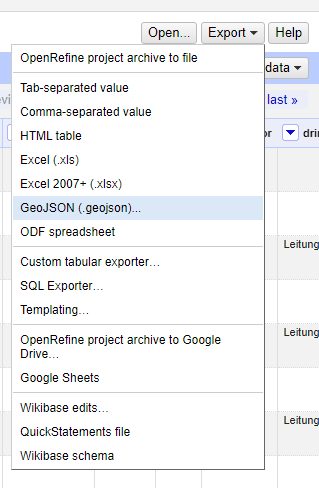
\includegraphics[width=7cm]{./Figures/GeoJSON_Export/geojson_export_button.png}
    \caption{The GeoJSON export button, located on the top right of an OpenRefine project}
\end{figure}

The dialog lets the user choose the name of the \textit{.geojson} file, the latitude/longitude columns, the WKT column
and the columns they want to include as properties of the geometry features. Latitude, longitude or WKT columns can be
ommitted from the export if such columns do not exist, however, if latitude or longitude columns are selected,
both of the columns are needed for a successful export (latitude and longitude).\\
\newline
The right side of the dialog lets the user choose what columns they want to include as properties to each of the GeoJSON features,
with the geometry columns selected on the left being ommitted from the properties table.\\
\newline
The user can also select the numeric scale of the decimal values of the geometries by tweaking the \textbf{Geometry numeric scale}
option at the bottom of the dialog to a different number, the default value is \texbf{7}. This number represents the
number of decimal digits to the right  of the decimal point of a decimal number, e.g. \textit{47.4955184} has a numeric scale of
7 because there are 7 numbers to the right of the decimal point of the number (this being the default numeric scale).
This numeric scale is used while processing lat/lon values or WKT values. \\
\newline
More information on what a numeric scale is can be found here:
\href{https://docs.microsoft.com/en-us/sql/t-sql/data-types/precision-scale-and-length-transact-sql?view=sql-server-ver15}{https://docs.microsoft.com/en-us/sql/t-sql/data-types/precision-scale-and-length-transact-sql?view=sql-server-ver15}.

\begin{figure}[H]
    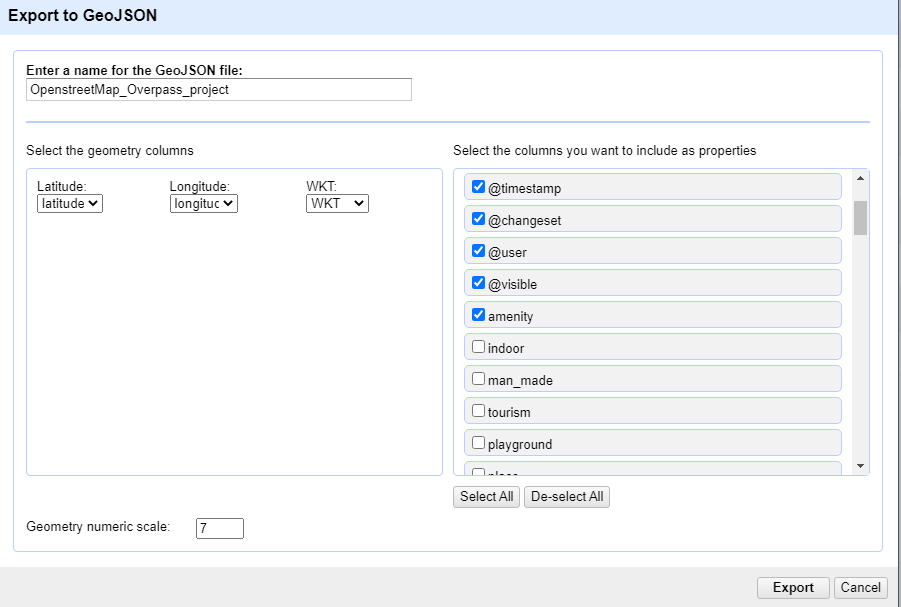
\includegraphics[width=\linewidth]{./Figures/GeoJSON_Export/geojson_export_dialog.png}
    \caption{The GeoJSON export dialog}
\end{figure}

\subsection{The Conversion Process}
\lipsum[15-17]
\subsection{Testing}
\lipsum[18-20]

\pagebreak
\section{Usage \& Examples}
\lipsum[9-10]
\subsection{Usage}
\lipsum[18-20]
\subsection{Examples}
\lipsum[3-4]